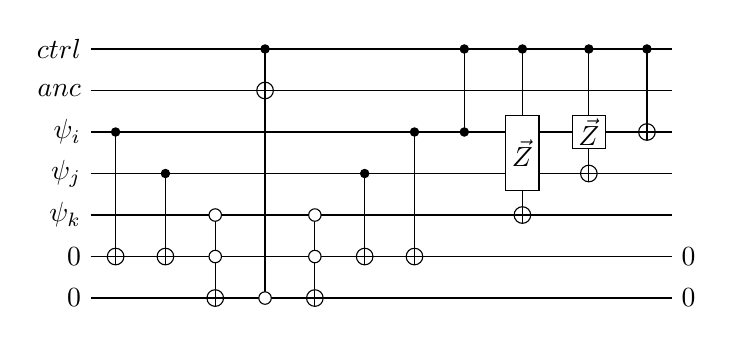
\begin{tikzpicture}[scale=1.000000,x=1pt,y=1pt]
\filldraw[color=white] (0.000000, -7.500000) rectangle (210.000000, 97.500000);
% Drawing wires
% Line 1: ctrl W ctrl
\draw[color=black] (0.000000,90.000000) -- (210.000000,90.000000);
\draw[color=black] (0.000000,90.000000) node[left] {$ctrl$};
% Line 2: anc W anc
\draw[color=black] (0.000000,75.000000) -- (210.000000,75.000000);
\draw[color=black] (0.000000,75.000000) node[left] {$anc$};
% Line 3: i W \psi_i
\draw[color=black] (0.000000,60.000000) -- (210.000000,60.000000);
\draw[color=black] (0.000000,60.000000) node[left] {$\psi_i$};
% Line 4: j W \psi_j
\draw[color=black] (0.000000,45.000000) -- (210.000000,45.000000);
\draw[color=black] (0.000000,45.000000) node[left] {$\psi_j$};
% Line 5: k W \psi_k
\draw[color=black] (0.000000,30.000000) -- (210.000000,30.000000);
\draw[color=black] (0.000000,30.000000) node[left] {$\psi_k$};
% Line 6: c0 W 0 0
\draw[color=black] (0.000000,15.000000) -- (210.000000,15.000000);
\draw[color=black] (0.000000,15.000000) node[left] {$0$};
% Line 7: c1 W 0 0
\draw[color=black] (0.000000,0.000000) -- (210.000000,0.000000);
\draw[color=black] (0.000000,0.000000) node[left] {$0$};
% Done with wires; drawing gates
% Line 9: i +c0
\draw (9.000000,60.000000) -- (9.000000,15.000000);
\filldraw (9.000000, 60.000000) circle(1.500000pt);
\begin{scope}
\draw[fill=white] (9.000000, 15.000000) circle(3.000000pt);
\clip (9.000000, 15.000000) circle(3.000000pt);
\draw (6.000000, 15.000000) -- (12.000000, 15.000000);
\draw (9.000000, 12.000000) -- (9.000000, 18.000000);
\end{scope}
% Line 10: j +c0
\draw (27.000000,45.000000) -- (27.000000,15.000000);
\filldraw (27.000000, 45.000000) circle(1.500000pt);
\begin{scope}
\draw[fill=white] (27.000000, 15.000000) circle(3.000000pt);
\clip (27.000000, 15.000000) circle(3.000000pt);
\draw (24.000000, 15.000000) -- (30.000000, 15.000000);
\draw (27.000000, 12.000000) -- (27.000000, 18.000000);
\end{scope}
% Line 11: -k -c0 +c1
\draw (45.000000,30.000000) -- (45.000000,0.000000);
\draw[fill=white] (45.000000, 30.000000) circle(2.250000pt);
\draw[fill=white] (45.000000, 15.000000) circle(2.250000pt);
\begin{scope}
\draw[fill=white] (45.000000, 0.000000) circle(3.000000pt);
\clip (45.000000, 0.000000) circle(3.000000pt);
\draw (42.000000, 0.000000) -- (48.000000, 0.000000);
\draw (45.000000, -3.000000) -- (45.000000, 3.000000);
\end{scope}
% Line 12: ctrl -c1 +anc
\draw (63.000000,90.000000) -- (63.000000,0.000000);
\filldraw (63.000000, 90.000000) circle(1.500000pt);
\draw[fill=white] (63.000000, 0.000000) circle(2.250000pt);
\begin{scope}
\draw[fill=white] (63.000000, 75.000000) circle(3.000000pt);
\clip (63.000000, 75.000000) circle(3.000000pt);
\draw (60.000000, 75.000000) -- (66.000000, 75.000000);
\draw (63.000000, 72.000000) -- (63.000000, 78.000000);
\end{scope}
% Line 13: -k -c0 +c1
\draw (81.000000,30.000000) -- (81.000000,0.000000);
\draw[fill=white] (81.000000, 30.000000) circle(2.250000pt);
\draw[fill=white] (81.000000, 15.000000) circle(2.250000pt);
\begin{scope}
\draw[fill=white] (81.000000, 0.000000) circle(3.000000pt);
\clip (81.000000, 0.000000) circle(3.000000pt);
\draw (78.000000, 0.000000) -- (84.000000, 0.000000);
\draw (81.000000, -3.000000) -- (81.000000, 3.000000);
\end{scope}
% Line 14: j +c0
\draw (99.000000,45.000000) -- (99.000000,15.000000);
\filldraw (99.000000, 45.000000) circle(1.500000pt);
\begin{scope}
\draw[fill=white] (99.000000, 15.000000) circle(3.000000pt);
\clip (99.000000, 15.000000) circle(3.000000pt);
\draw (96.000000, 15.000000) -- (102.000000, 15.000000);
\draw (99.000000, 12.000000) -- (99.000000, 18.000000);
\end{scope}
% Line 15: i +c0
\draw (117.000000,60.000000) -- (117.000000,15.000000);
\filldraw (117.000000, 60.000000) circle(1.500000pt);
\begin{scope}
\draw[fill=white] (117.000000, 15.000000) circle(3.000000pt);
\clip (117.000000, 15.000000) circle(3.000000pt);
\draw (114.000000, 15.000000) -- (120.000000, 15.000000);
\draw (117.000000, 12.000000) -- (117.000000, 18.000000);
\end{scope}
% Line 17: ctrl i
\draw (135.000000,90.000000) -- (135.000000,60.000000);
\filldraw (135.000000, 90.000000) circle(1.500000pt);
\filldraw (135.000000, 60.000000) circle(1.500000pt);
% Line 19: i j G $\vec{Z}$ ctrl +k
\draw (156.000000,90.000000) -- (156.000000,30.000000);
\begin{scope}
\draw[fill=white] (156.000000, 52.500000) +(-45.000000:8.485281pt and 19.091883pt) -- +(45.000000:8.485281pt and 19.091883pt) -- +(135.000000:8.485281pt and 19.091883pt) -- +(225.000000:8.485281pt and 19.091883pt) -- cycle;
\clip (156.000000, 52.500000) +(-45.000000:8.485281pt and 19.091883pt) -- +(45.000000:8.485281pt and 19.091883pt) -- +(135.000000:8.485281pt and 19.091883pt) -- +(225.000000:8.485281pt and 19.091883pt) -- cycle;
\draw (156.000000, 52.500000) node {$\vec{Z}$};
\end{scope}
\filldraw (156.000000, 90.000000) circle(1.500000pt);
\begin{scope}
\draw[fill=white] (156.000000, 30.000000) circle(3.000000pt);
\clip (156.000000, 30.000000) circle(3.000000pt);
\draw (153.000000, 30.000000) -- (159.000000, 30.000000);
\draw (156.000000, 27.000000) -- (156.000000, 33.000000);
\end{scope}
% Line 20: i G $\vec{Z}$ ctrl +j
\draw (180.000000,90.000000) -- (180.000000,45.000000);
\begin{scope}
\draw[fill=white] (180.000000, 60.000000) +(-45.000000:8.485281pt and 8.485281pt) -- +(45.000000:8.485281pt and 8.485281pt) -- +(135.000000:8.485281pt and 8.485281pt) -- +(225.000000:8.485281pt and 8.485281pt) -- cycle;
\clip (180.000000, 60.000000) +(-45.000000:8.485281pt and 8.485281pt) -- +(45.000000:8.485281pt and 8.485281pt) -- +(135.000000:8.485281pt and 8.485281pt) -- +(225.000000:8.485281pt and 8.485281pt) -- cycle;
\draw (180.000000, 60.000000) node {$\vec{Z}$};
\end{scope}
\filldraw (180.000000, 90.000000) circle(1.500000pt);
\begin{scope}
\draw[fill=white] (180.000000, 45.000000) circle(3.000000pt);
\clip (180.000000, 45.000000) circle(3.000000pt);
\draw (177.000000, 45.000000) -- (183.000000, 45.000000);
\draw (180.000000, 42.000000) -- (180.000000, 48.000000);
\end{scope}
% Line 21: ctrl +i
\draw (201.000000,90.000000) -- (201.000000,60.000000);
\filldraw (201.000000, 90.000000) circle(1.500000pt);
\begin{scope}
\draw[fill=white] (201.000000, 60.000000) circle(3.000000pt);
\clip (201.000000, 60.000000) circle(3.000000pt);
\draw (198.000000, 60.000000) -- (204.000000, 60.000000);
\draw (201.000000, 57.000000) -- (201.000000, 63.000000);
\end{scope}
% Done with gates; drawing ending labels
\draw[color=black] (210.000000,15.000000) node[right] {$0$};
\draw[color=black] (210.000000,0.000000) node[right] {$0$};
% Done with ending labels; drawing cut lines and comments
% Done with comments
\end{tikzpicture}
